\documentclass[10pt,spanish,a4paper,openany,notitlepage]{article}
%-------------------------------------Paquetes-----------------------------------------------------------------------
\usepackage[spanish,es-tabla]{babel}  	% Traduce los textos a castellano
\usepackage[utf8]{inputenc}	% Permite escribir directamente áéíóúñ
\usepackage{t1enc}            	% Agrega caracteres extendidos al font
\usepackage{amsmath} 		%Permite imprimir mas opcciones matematicas
\usepackage{graphicx}		%Permite agregar imagenes al informe
\usepackage{multicol}  		%Permite dividir el texto en varias columnas
\usepackage{float} 		%Permite utilizar H para colocar las imagenes en un lugar especifico 
\usepackage{units}
\usepackage{circuitikz}
\usepackage{caption}
\usepackage{subcaption}
\usepackage{sidecap}
\usepackage{mathtools}
\usepackage{multirow} % Paquete para dividir las tablas en subtablas
\usepackage{booktabs} %estos 2 sirven para achicar la tabla
\usepackage{tabulary}
\usepackage{fancyhdr} % encabezado
\usepackage{textcomp} % para usar ° con el comando \textdegree
\usepackage{anysize}		%Permite modificar los margenes del documento
\usepackage{abstract} % paquete para el resumen del articulo
 
%---------------------------------------Configuraciones de pagina----------------------------------------------
\marginsize{2.5cm}{2.5cm}{1cm}{1cm}

\pagestyle{fancy}
\fancyhf{}
\lhead{
66.25 - \textsc{Dispositivos Semiconductores}\\ 
2\textsuperscript{do} Cuatrimestre de 2014
}
\rhead{
\includegraphics[width=3cm]{imagenes/FIUBA_ALTA.jpg}}
\rfoot{Página \thepage}

%---------------------------------------Definiciones propias---------------------------------------------------------
\newcommand{\oiint}{\displaystyle\bigcirc\!\!\!\!\!\!\!\!\int\!\!\!\!\!\int} %Integral doble cerrada

\DeclarePairedDelimiter\abs{\lvert}{\rvert}%
\DeclarePairedDelimiter\norm{\lVert}{\rVert}%
% Swap the definition of \abs* and \norm*, so that \abs
% and \norm resizes the size of the brackets, and the 
% starred version does not.
\makeatletter
\let\oldabs\abs
\def\abs{\@ifstar{\oldabs}{\oldabs*}}
%
\let\oldnorm\norm
\def\norm{\@ifstar{\oldnorm}{\oldnorm*}}
\makeatother
%--------------------------------------------------------------------------------------------------------------------------------


\makeatletter
\let\ps@plain\ps@fancy 
\makeatother

% lo siguiente es para borrar el titulo del resumen y que no ocupe espacio:
 \AtBeginDocument{%
 \renewcommand{\abstractname}{}%
 }
\renewcommand{\absnamepos}{empty} % originally center
 

\begin{document}
\title{\textbf{TP N\textdegree2: Curvas características del transistor TBJ BC548C}}
\author{
  Accifonte, Franco - 93799\\
  \texttt{franco.accifonte@gmail.com}  
  \and
  Iturria, Germán  - 86270 \\
  \texttt{german.iturria@gmail.com}
  \and
   Vázquez, Matías - 91523\\
  \texttt{mfvazquez@gmail.com}
}
\date{30 de octubre de 2014}
\maketitle

\begin{abstract} %Resumen
\emph{En el siguiente trabajo se analizan las principales características 
de polarización y frecuencias medias de transistores TBJ tipo NPN. 
Estudiando las curvas de transferencia y de salida, obtenidas en mediciones, 
se consiguen los parámetros característicos y se calculan los parámetros 
de pequeña señal. Finalmente se realiza un modelo básico de Spice con los 
parámetros calculados y se presentan simulaciones para contrastar con las mediciones.}
\end{abstract}

\section{Desarrollo}

A continuación se detalla el desarrollo del trabajo realizado, tanto la 
realización de las simulaciones mediantes \emph{Spice}, como las mediciones realizadas.

\subsection{Simulación de transistores BC548C}

En primera instancia se obtuvieron con \emph{LTSPICE} las curvas de transferencia, 
la ganancia de corriente entre base y colector y las curvas de salida  propias al transistor. Usando las bibliotecas  
 \texttt{PHIL\_BJT} y \texttt{SIEMENS} proporcionadas por la cátedra.

\subsubsection{Curva de transferencia}

Se simuló $I_C$ vs. $V_{BE}$ para $V_{CE} = 1,25 \unit{V}$ para ambas 
bibliotecas. Se varió la tensión $V_{BE}$ entre $0\unit{V}$ y $0,9\unit{V}$ 
con pasos de $0,01\unit{V}$, utilizando el circuito simulado en la figura \ref{circuito:simulacion_transferencia}.

\begin{figure}[H]
\centering
\begin{circuitikz}[american]\shorthandoff{>}
\draw 
(1.5,2) node[npn](npn){BC548C}
(0,0.5)  node[ground]{} to [V, l=$V_{BE}$] (0,2) -- (npn.base)
(1.5,0.5)node[ground]{} -- (npn.emitter) 
(3,0.5)  node[ground]{} to [V, l_= $V_{CE}$] (3,2.77) -- (npn.collector)
;\end{circuitikz}
\caption{Circuito utilizado para la simulación de las curvas de transferencia.}
\label{circuito:simulacion_transferencia}
\end{figure}

\subsubsection{Ganancia de corriente entre base y colector}

Para ambas bibliotecas se simuló el circuito de la figura \ref{circuito:simulacion_ganancia_salida} 
bajo las condiciones de medición del multímetro que se utilizará en las mediciones. 
Estas son $I_B = 10\unit{\mu A}$ y $V_{CE} = 2,8\unit{V}$. Se obtuvo el parámetro \texttt{BETADC} del \texttt{Simulation Output File}.

\begin{figure}[H]
\centering
\begin{circuitikz}[american]\shorthandoff{>}
\draw 
(1.5,2) node[npn](npn){BC548C}
(0,0.5)  node[ground]{} to [I, l=$I_{B}$] (0,2) -- (npn.base)
(1.5,0.5)node[ground]{} -- (npn.emitter) 
(3,0.5)  node[ground]{} to [V, l_= $V_{CE}$] (3,2.77) -- (npn.collector)
;\end{circuitikz}
\caption{Circuito utilizado para la simulación de las curvas de salida y de la ganancia de corriente.}
\label{circuito:simulacion_ganancia_salida}
\end{figure}

Se obtuvieron los siguientes valores:

\begin{itemize}
\item{\texttt{PHIL\_BJT}}: $h_{FE} = 460$
\item{\texttt{SIEMENS}}: $h_{FE} = 432$
\end{itemize}

\subsubsection{Curva de salida}

Se simuló $I_C$ vs. $V_{CE}$ para $I_{B} = cte$ para ambas bibliotecas. Se varió la 
tensión $V_{CE}$ entre $0\unit{V}$ y $5\unit{V}$ con pasos de $0,01\unit{V}$, 
utilizando el circuito simulado en la figura \ref{circuito:simulacion_ganancia_salida}.

La corriente $I_B$ se determinó mediante la ecuación \ref{eq:I_B} para cada valor 
de $I_C$ deseado, utilizando el parámetro $h_{FE}$ correspondiente al transistor de cada biblioteca. 

\begin{equation}
I_B = \frac{I_C}{h_{FE}}
\label{eq:I_B}
\end{equation}

A continuación se listan los valores de $I_B$ utilizados.

\begin{itemize}
\item{\texttt{PHIL\_BJT} con $h_{FE} = 460$}
\begin{itemize}
\item{$I_C = 5 \unit{mA}$}: $I_B = 10,9\unit{\mu A}$
\item{$I_C = 25 \unit{mA}$}: $I_B = 54,3\unit{\mu A}$
\end{itemize}
\item{\texttt{SIEMENS} con $h_{FE} = 432$}
\begin{itemize}
\item{$I_C = 5 \unit{mA}$}: $I_B = 11,6\unit{\mu A}$
\item{$I_C = 25 \unit{mA}$}: $I_B = 57,9\unit{\mu A}$
\end{itemize}
\end{itemize}

\subsection{Obtención de parámetros de las hojas de datos}

De la hoja de datos de MCC(Micro Commercial Components) se obtuvieron los siguientes valores:

\begin{itemize}
\item $h_{FE} =300 $
\item $I_S = 8,4 \unit{fA}$
\item $0,55 \unit{V} \leq V_{BE(ON)} \leq 0,7 \unit{V}$
\item $V_{CE(SAT)} = 0,3 \unit{V}$
\item $V_A = 100 \unit{V}$
\item $g_m = 0,487 \Omega^{-1}$
\end{itemize}

De la hoja de datos de Siemens se obtuvieron los siguientes valores:

\begin{itemize}
\item $h_{FE} =270$
\item $I_S = 171,4 \unit{fA}$
\item $V_{BE(ON)} = 0,66\unit{V}$
\item $V_{CE(SAT)} = 0,3 \unit{V}$
\item $V_A = 100 \unit{V}$
\item $g_m = 2 \Omega^{-1}$
\end{itemize}

\subsection{Obtención de las curvas de forma experimental}

Se obtuvieron las curvas de tres transistores \textbf{TBJ BC548C} distintos 
utilizando una placa experimental, reguladores de tensión \textbf{LM317} y 
 \textbf{LM7805}, un potenciómetro lineal de $20\unit{k\Omega}$ y resistencias de valores apropiados para cada medición.
También se midió para cada transistor el valor de $h_{FE}$ utilizando un multímetro con esta función.

\subsubsection{Curva de transferencia}

Para obtener la curva $I_C$ vs $V_{BE}$ se utilizó el banco de mediciones 
presentado en la figura \ref{circuito:medicion_transferencia}. El regulador de 
tensión \textbf{LM317} fija la tensión $V_{CE}=1,25\unit{V}$ y el regulador de 
tensión \textbf{LM7805} provee una alimentación constante de $5\unit{V}$. 
El potenciómetro utilizado es de $20 \unit{k\Omega}$.

\begin{figure}[H] %[h] para here [b] para bottom [t] para top [H]+float para aqui si o si
\begin{center}
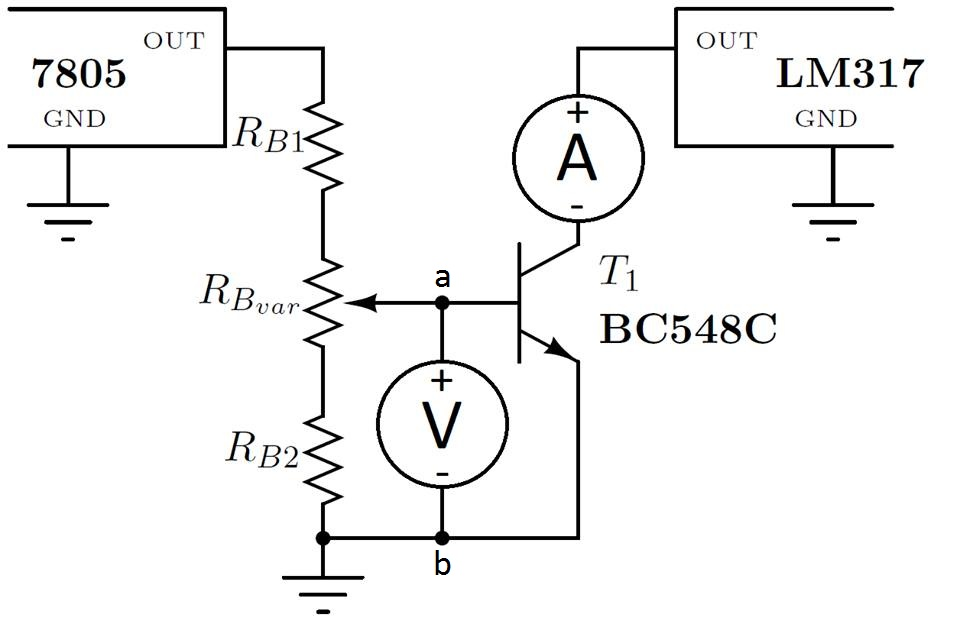
\includegraphics[scale=0.3]{./imagenes/ic_vbe.jpg}
\caption{Circuito para la medición de la curva de transferencia $I_C$ vs. $V_{BE}$}
 \label{circuito:medicion_transferencia}
\end{center}
\end{figure}

Para la obtención de las resistencias $R_{B1}$ y $R_{B2}$ se partió 
planteando el rango de la corriente $I_C$ deseado y suponiendo $h_{FE} = 200$ 
se obtuvo el rango de $I_B$.

\[ \displaystyle 0 \unit{mA} \leq I_C \leq 50\unit{mA} \ \ \ \ \ \Longrightarrow \ \ \ \ \  0 \unit{\mu A} \leq I_B \leq 250 \unit{\mu A} \]

Luego se obtuvo el equivalente de Thévenin entre los terminales $a$ y $b$. 
Para simplificar las ecuaciones se utilizó $R_1 = R_{B1} + R_{B1_{var}}$ y 
$R_2 = R_{B2} + R_{B2_{var}}$ con $R_{B_{var}} = R_{B1_{var}} + R_{B2_{var}} = 20 \unit{k\Omega}$. 
Siendo $R_{B_{var}}$ el potenciometro de $20 \unit{k\Omega}$.

\[ \displaystyle V_{TH} = V_{DD} \frac{R_1}{R_1 + R_2}\ \ \ \ \ \ \ \ \ \ R_{TH} = \frac{R_1\ R_2}{R_1 + R_2}\]

Siendo $V_{DD}$ la salida del regulador de tensión \textbf{LM7805}. 

Del circuito mostrado en la figura \ref{circuito:medicion_transferencia} 
obtenemos la ecuación \ref{eq:I_B}

\begin{equation}
\displaystyle I_B = \frac{V_{TH} - V_{BE_{ON}}}{R_{TH}}
\label{eq:I_B}
\end{equation}

Reemplazando la ecuación \ref{eq:I_B} en el rango de valores deseado.

Para el mínimo valor de $I_B$:

\[ \displaystyle \frac{V_{TH} - V_{BE_{ON}}}{R_{TH}} \geq 0 \unit{\mu A} \]

Entonces:

\begin{equation}
V_{TH} \geq V_{BE_{ON}}
\label{eq:Vth_baja}
\end{equation}

Para el máximo valor de $I_B$:

\begin{equation}
\frac{V_{TH} - V_{BE_{ON}}}{R_{TH}} \leq 250 \unit{\mu A}
\label{eq:Vth_alta}
\end{equation}

Con las inecuaciones \ref{eq:Vth_baja} y \ref{eq:Vth_alta} se buscaron 
valores de $R_{B1}$ y $R_{B2}$ que las cumplan. Teniendo en cuenta que 
para cada inecuación los valores de $V_{TH}$ y $R_{TH}$ son distintos ya 
que dependen de $R_1$ y $R_2$ que varían por estar conectados a un 
potenciómetro y $0,5 \unit{V} \leq V_{BE_{ON}} \leq 0,7 \unit{V}$.\\

Se propusieron los siguientes valores $R_{B1} = 5\unit{k\Omega}$ y $R_{B2} = 25\unit{k\Omega}$:

\begin{itemize}
\item{Para $I_B \geq 0 \unit{\mu A}$}: $V_{BE_{ON}} = 0,5 \unit{V}$, $R_1 = R_{B1} = 5 \unit{k\Omega}$ y $R_2 = R_{B2} + 20\unit{k\Omega} = 45 \unit{k\Omega}$

Obteniendo los siguientes valores para el equivalente de Thévenin:

\[ \displaystyle V_{TH} =  0,5 \unit{V} \geq 0,5 \unit{V} = V_{BE_{ON}}\]

\item{Para $I_B \leq 250 \unit{\mu A}$}: $V_{BE_{ON}} = 0,7 \unit{V}$, $R_1 = R_{B1}+ 20\unit{k\Omega} = 25 \unit{k\Omega}$ y $R_2 = R_{B2} = 25 \unit{k\Omega}$

\[ \displaystyle V_{TH} =  2,5 \unit{V} \ \ \ \ \ \ \ \ \ \  R_{TH} = 12,5 \unit{k\Omega}\]

\[ \displaystyle \frac{V_{TH} - V_{BE_{ON}}}{R_{TH}} = \frac{2,5 \unit{V} - 0,7 \unit{V}}{12,5 \unit{k\Omega}} = 144 \unit{\mu A} \leq 250 \unit{\mu A} \]

Entonces el valor máximo medido de $I_C$ será: $I_{C_{MAX}} = I_B\ h_{FE} = 144 \unit{\mu A}\ 200 = 28,8 \unit{mA}$

\end{itemize}

Como se ve los valores $R_{B1}$ y $R_{B2}$ elegidos cumplen las condiciones esperadas.

\subsubsection{Ganancia de corriente entre base y colector}

Para obtener $h_{FE}$ se utilizó un multímetro que realiza la medición 
bajo las condiciones $I_B = 10 \unit{\mu A}$ y $V_{CE} = 2,8 \unit{V}$

Se obtuvieron los siguientes valores para cada transistor:

\begin{itemize}
\item{Transistor 1:} $h_{FE} = 361$
\item{Transistor 2:} $h_{FE} = 326$
\item{Transistor 3:} $h_{FE} = 253$
\end{itemize}

\subsubsection{Curva de salida}

Para obtener la curva $i_C$ vs $v_{CE}$ se utilizó el banco de mediciones 
presentado en la figura \ref{circuito:medicion_salida}.El regulador de 
tensión \textbf{LM7805} provee una alimentación constante de $5\unit{V}$. 
El potenciómetro utilizado es de $20 \unit{k\Omega}$.

\begin{figure}[H] %[h] para here [b] para bottom [t] para top [H]+float para aqui si o si
\begin{center}
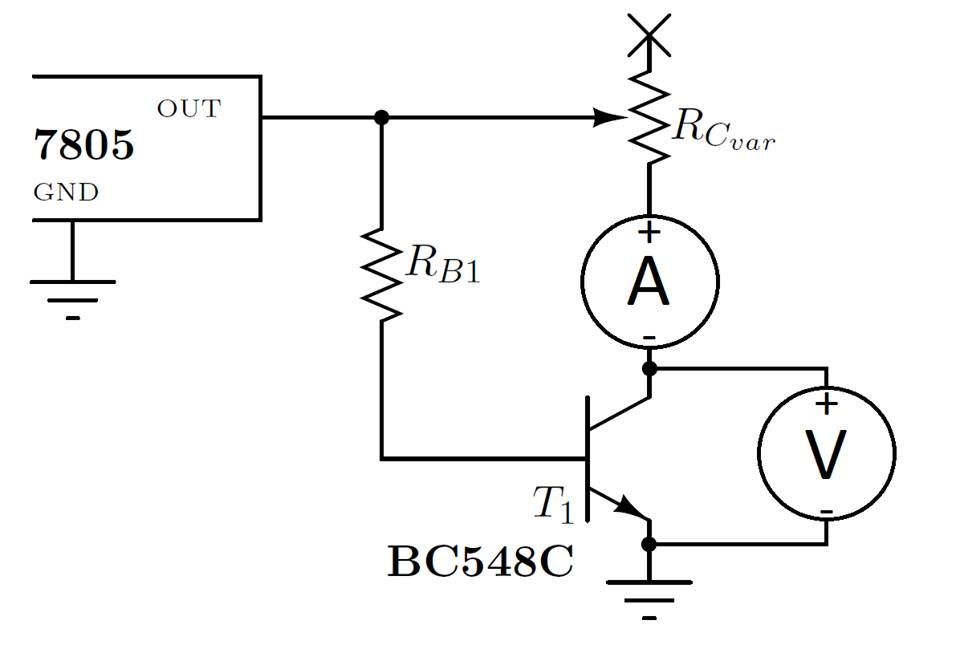
\includegraphics[scale=0.2]{./imagenes/ic_vce.jpg}
\caption{Circuito para la medición de la curva de salida $I_C$ vs. $V_{CE}$}
 \label{circuito:medicion_salida}
\end{center}
\end{figure}

Para la obtención de la resistencia $R_{B1}$ planteamos la ecuación obtenida 
del circuito mostrado en la figura \ref{circuito:medicion_salida}:

\[ \displaystyle R_{B1} = \frac{V_{DD} - V_{BE_{ON}}}{I_B} \]


Y teniendo en cuenta que $I_B = \frac{I_C}{h_{fe}}$ se llegó a la ecuación \ref{eq:RB1}

\begin{equation}
R_{B1} = \frac{(V_{DD} - V_{BE_{ON}}) h_{FE}}{I_C}
\label{eq:RB1}
\end{equation}

Siendo $V_{DD} = 5 \unit{V}$ la salida del regulador de tensión  \textbf{LM7805} y $V_{BE_{ON}} = 0,7 \unit{V}$

A continuación listamos los valores de $R_{B1}$ para cada transistor y para cada $I_C$:

\begin{itemize}

\item{Transistor 1:} $h_{FE} = 361$

\begin{itemize}
\item{Para $I_C = 5 \unit{mA}$}: $R_{B1} \approx 310 \unit{k\Omega}$
\item{Para $I_C = 25 \unit{mA}$}: $R_{B1} \approx  62\unit{k\Omega}$
\end{itemize}

\item{Transistor 2:} $h_{FE} = 326$

\begin{itemize}
\item{Para $I_C = 5 \unit{mA}$}: $R_{B1} \approx  280\unit{k\Omega}$
\item{Para $I_C = 25 \unit{mA}$}: $R_{B1} \approx  56\unit{k\Omega}$
\end{itemize}

\item{Transistor 3:} $h_{FE} = 253$

\begin{itemize}
\item{Para $I_C = 5 \unit{mA}$}: $R_{B1} \approx  217\unit{k\Omega}$
\item{Para $I_C = 25 \unit{mA}$}: $R_{B1} \approx  43\unit{k\Omega}$
\end{itemize}

\end{itemize}

\subsection{Obtención de parámetros a partir de las mediciones}

\subsubsection{Parámetros característicos}

En las curvas de transferencia $I_C$ vs. $V_{BE}$ medidas y simuladas se 
obtuvieron los parámetros $I_S$ y $V_{th}$ mediante un ajuste. Se utilizaron 
dos métodos de ajuste distintos.\\

\textbf{Ajuste exponencial:} Se tomaron los resultados de la expresión

\[ \displaystyle I_C  = I_S\ e^{\frac{V_{BE}}{V_{th}}} \]

y se realizó un ajuste mediante una función exponencial.

\[ \displaystyle y  = A\ e^{B x} \]

\textbf{Ajuste lineal:} Se tomaron los resultados de la expresión

\[ \displaystyle ln(I_C)  = ln(I_S) + \frac{V_{BE}}{V_{th}} \]

y se realizó un ajuste mediante una recta.

\[ \displaystyle y  = A x + B \]

En las curvas de salida $I_C$ vs. $V_{CE}$ medidas y simuladas se obtuvieron 
los parámetros $I_{C_{sat}}$ y $r_o$ mediante un ajuste lineal, en la región 
de modo activo directo, a los resultados de la expresión

\[ \displaystyle I_C  = I_{C_{sat}} + \frac{V_{CE}}{r_o} \]

Luego pudo ser calculada la \emph{Tensión de Early} $V_A$ mediante la expresión

\[ \displaystyle V_A = r_o I_{C_{sat}} \]

\subsubsection{Cálculo de parámetros de pequeña señal}

Se calculó y graficó $g_m$ en función de la corriente $I_C$ como

\[ \displaystyle g_m(k) = \frac{I_C(k) - I_C(k-1)}{V_{BE}(k)-V_{BE}(k-1)} \]

Tanto para los transistores simulados como los utilizados en la medición experimental.

Mediante cálculos teóricos, utilizando los parámetros obtenidos en los ajustes, se obtuvo la siguiente ecuación

\[ \displaystyle  g_m = \frac{\displaystyle \partial i_{C}}{\displaystyle \partial v_{BE}}\Bigr\rfloor_Q = \frac{\displaystyle I_S}{\displaystyle V_{th}} e^{\frac{\displaystyle V_{BE}}{\displaystyle V_{th}}} = \frac{\displaystyle I_C}{\displaystyle V_{th}} \]

Para los 3 transistores utilizados en la medición experimental.\\

Finalmente se graficó $r_\pi$ mediante la siguiente ecuación

\[ \displaystyle r_\pi = \frac{h_{FE}}{g_m} \]

Utilizando los distintos todos los $g_m$ obtenidos mediante los dos métodos 
antes mencionados.

\subsection{Simulación del modelo modificado}

Se diseñó un modelo modificado basado en el modelo de \emph{Spice} del 
TBJ NPN genérico ajustado a los parámetros característicos del Transistor 1. 
Realizamos las mismas simulaciones que para las bibliotecas \texttt{PHIL\_BJT} 
y \texttt{SIEMENS} incluyendo la siguiente directiva:\\

\texttt{.MODEL MiModelo NPN (BF=361 IS=106.239f VAF=86.67009)}\\

Para la simulación de la ganancia de corriente entre base y colector se obtuvo $h_{FE} = 370$

\section{Análisis y comparación de los resultados}

\subsection{Curvas obtenidas}

\begin{figure}[H] %[h] para here [b] para bottom [t] para top [H]+float para aqui si o si
\begin{center}
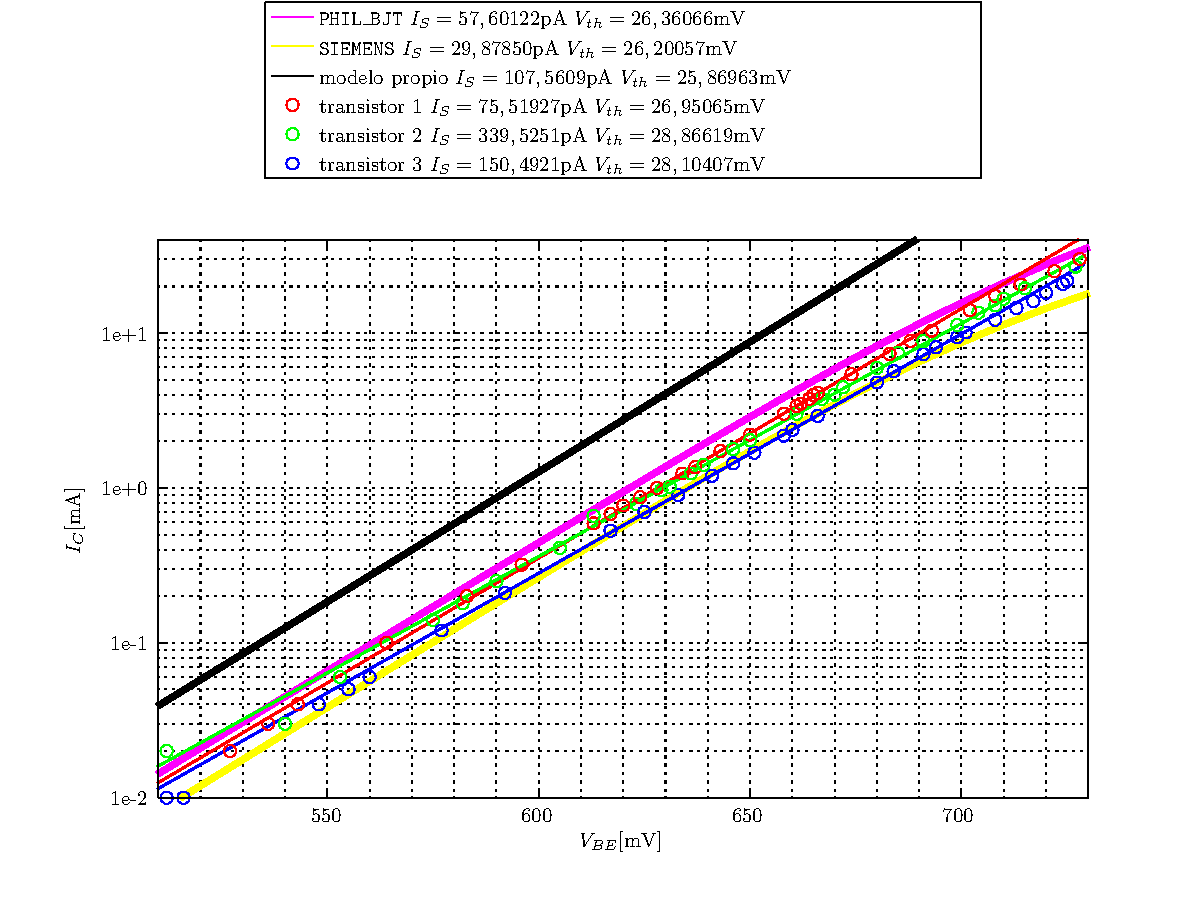
\includegraphics[scale=0.7]{./Octave/IdvsVbe_exp.pdf}
\caption{Curva de transferencia con ajuste exponencial}
 \label{fig:transferencia_exp}
\end{center}
\end{figure}

\begin{figure}[H] %[h] para here [b] para bottom [t] para top [H]+float para aqui si o si
\begin{center}
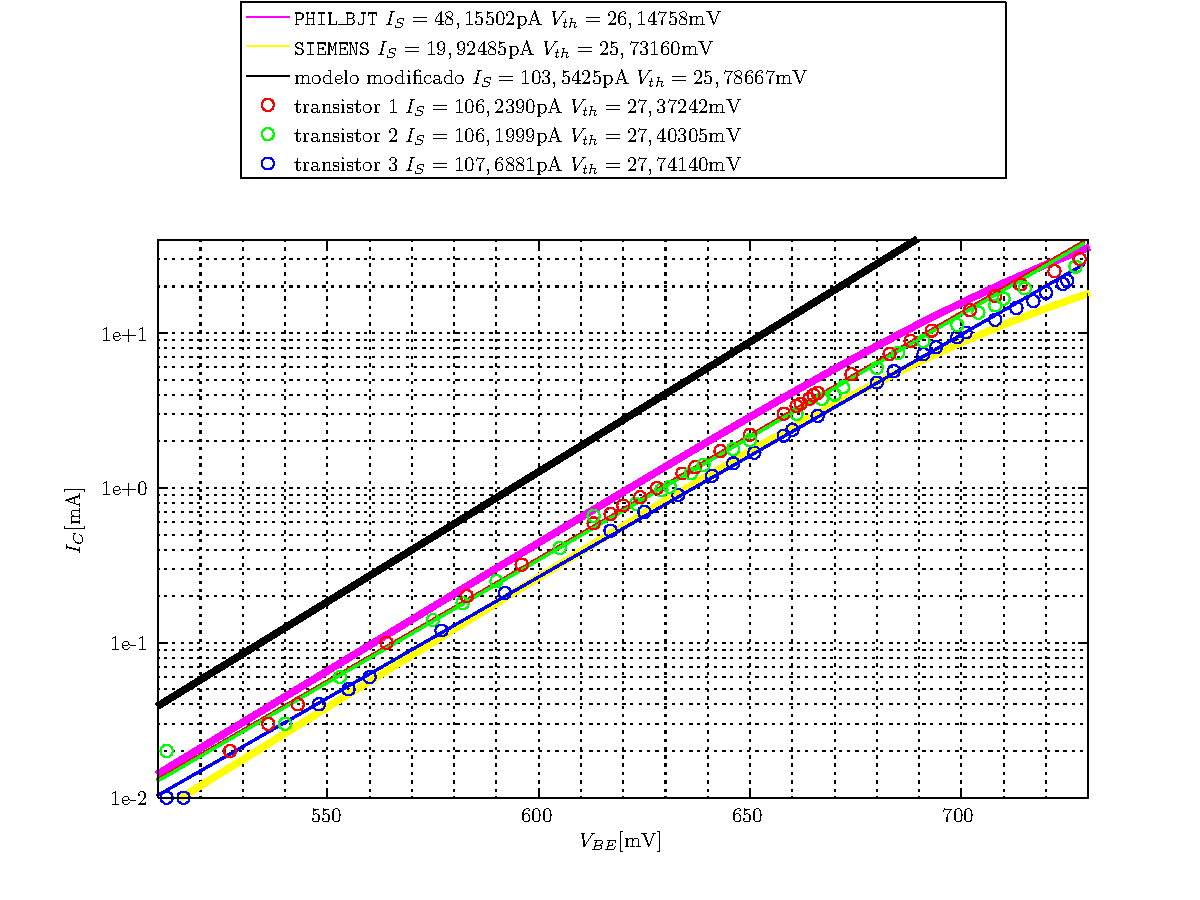
\includegraphics[scale=0.7]{./Octave/IdvsVbe_recta.pdf}
\caption{Curva de transferencia con ajuste lineal}
 \label{fig:transferencia_lineal}
\end{center}
\end{figure}

\begin{figure}[H] %[h] para here [b] para bottom [t] para top [H]+float para aqui si o si
\begin{center}
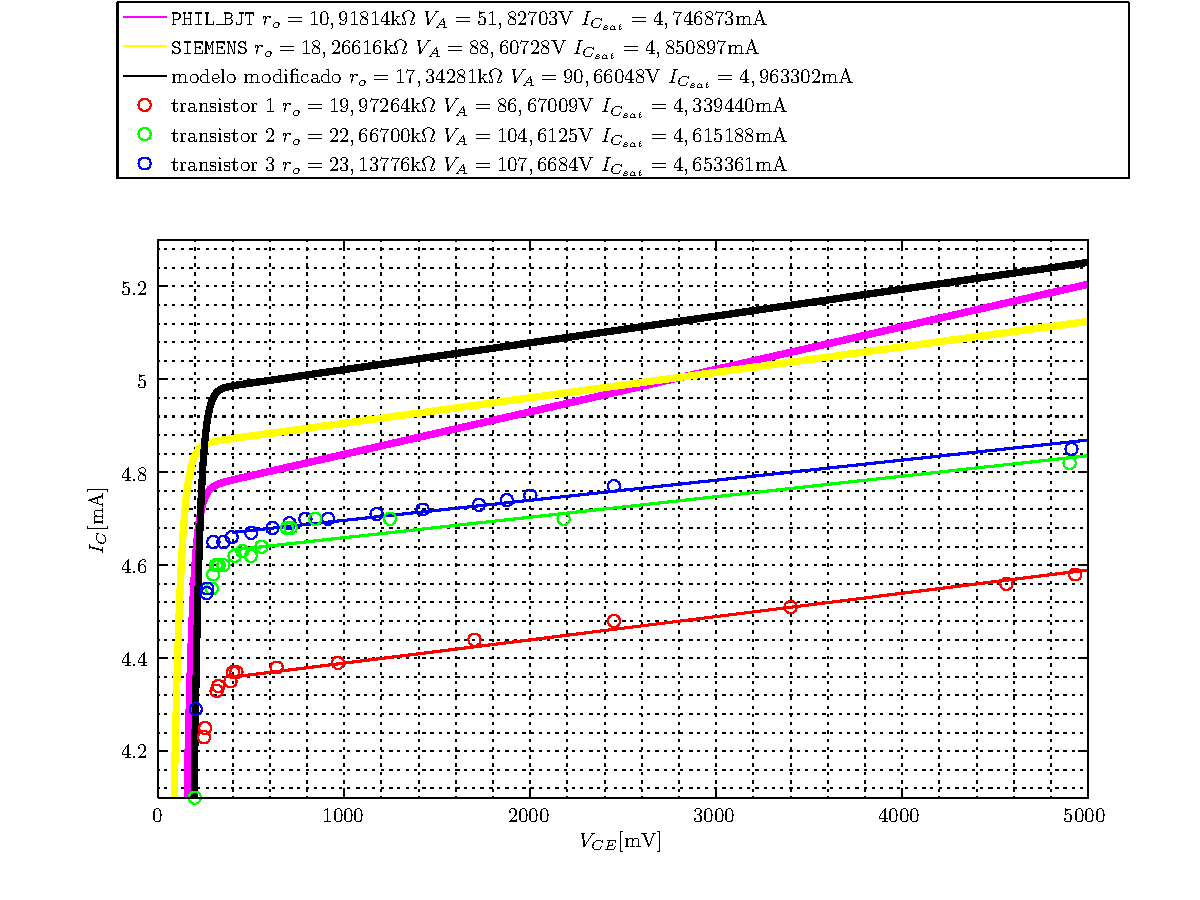
\includegraphics[scale=0.7]{./Octave/IcvsVce_5mA.pdf}
\caption{Curva de salida para $I_{C_{MAD}} = 5\unit{mA}$}
 \label{fig:salida_5ma}
\end{center}
\end{figure}

\begin{figure}[H] %[h] para here [b] para bottom [t] para top [H]+float para aqui si o si
\begin{center}
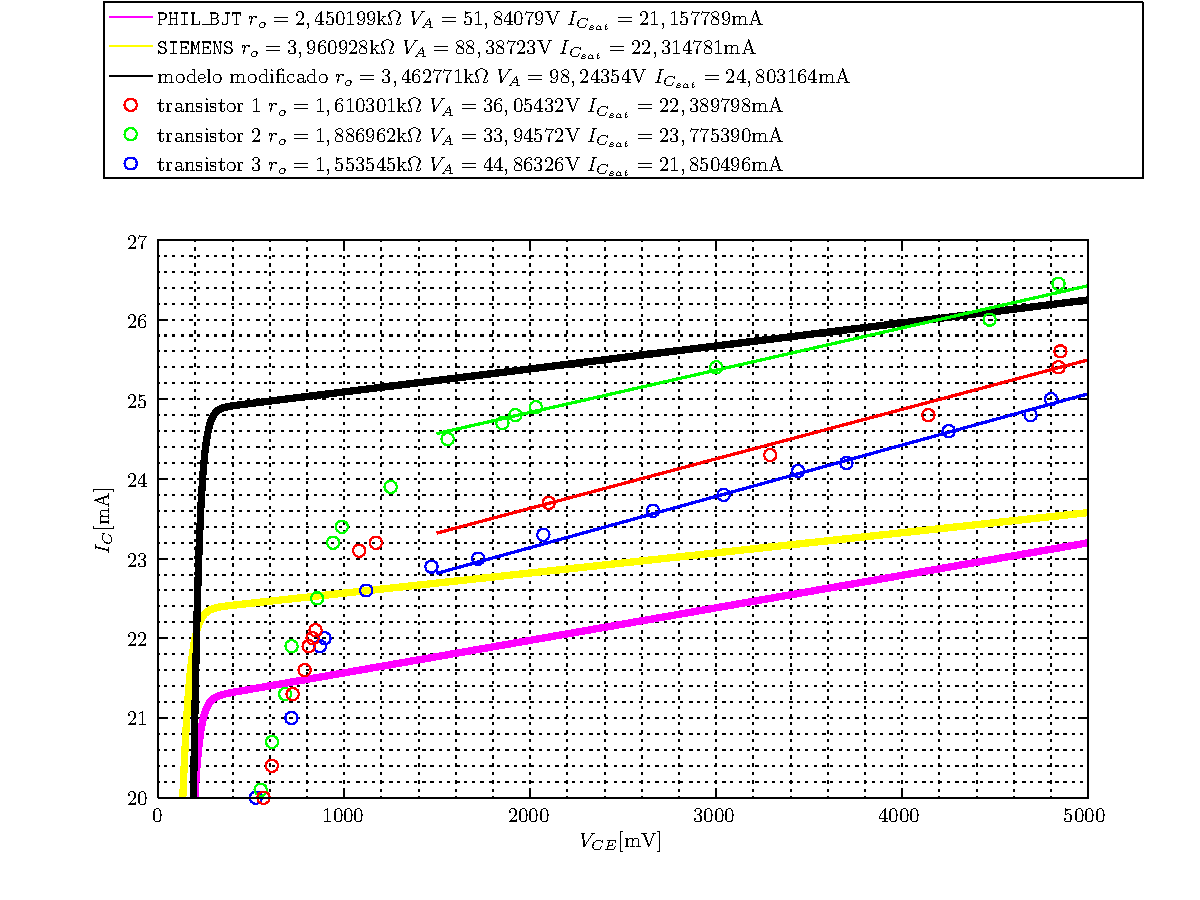
\includegraphics[scale=0.7]{./Octave/IcvsVce_25mA.pdf}
\caption{Curva de salida para $I_{C_{MAD}} = 25\unit{mA}$}
 \label{fig:salida_25ma}
\end{center}
\end{figure}

\begin{figure}[H] %[h] para here [b] para bottom [t] para top [H]+float para aqui si o si
\begin{center}
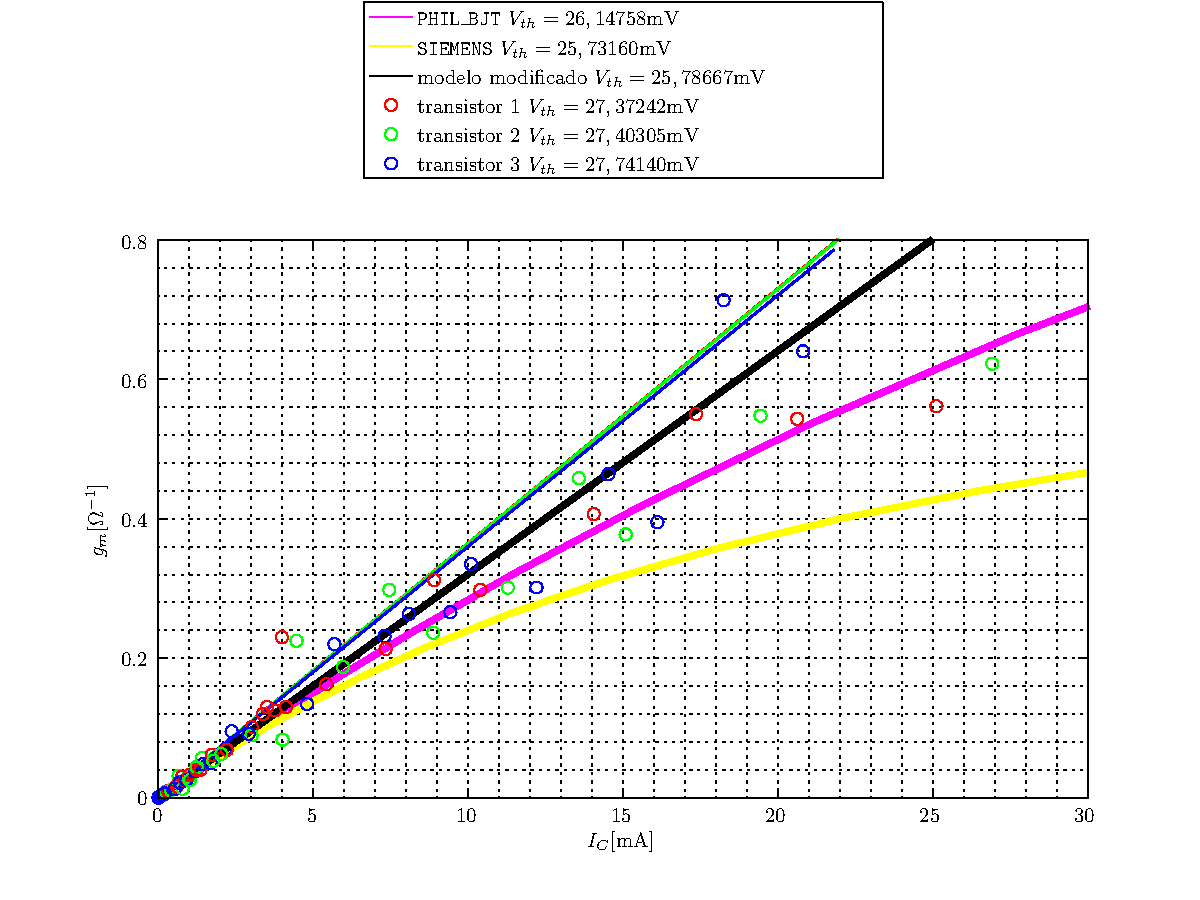
\includegraphics[scale=0.7]{./Octave/gm.pdf}
\caption{Curva de transconductancia}
 \label{fig:gm}
\end{center}
\end{figure}

\begin{figure}[H] %[h] para here [b] para bottom [t] para top [H]+float para aqui si o si
\begin{center}
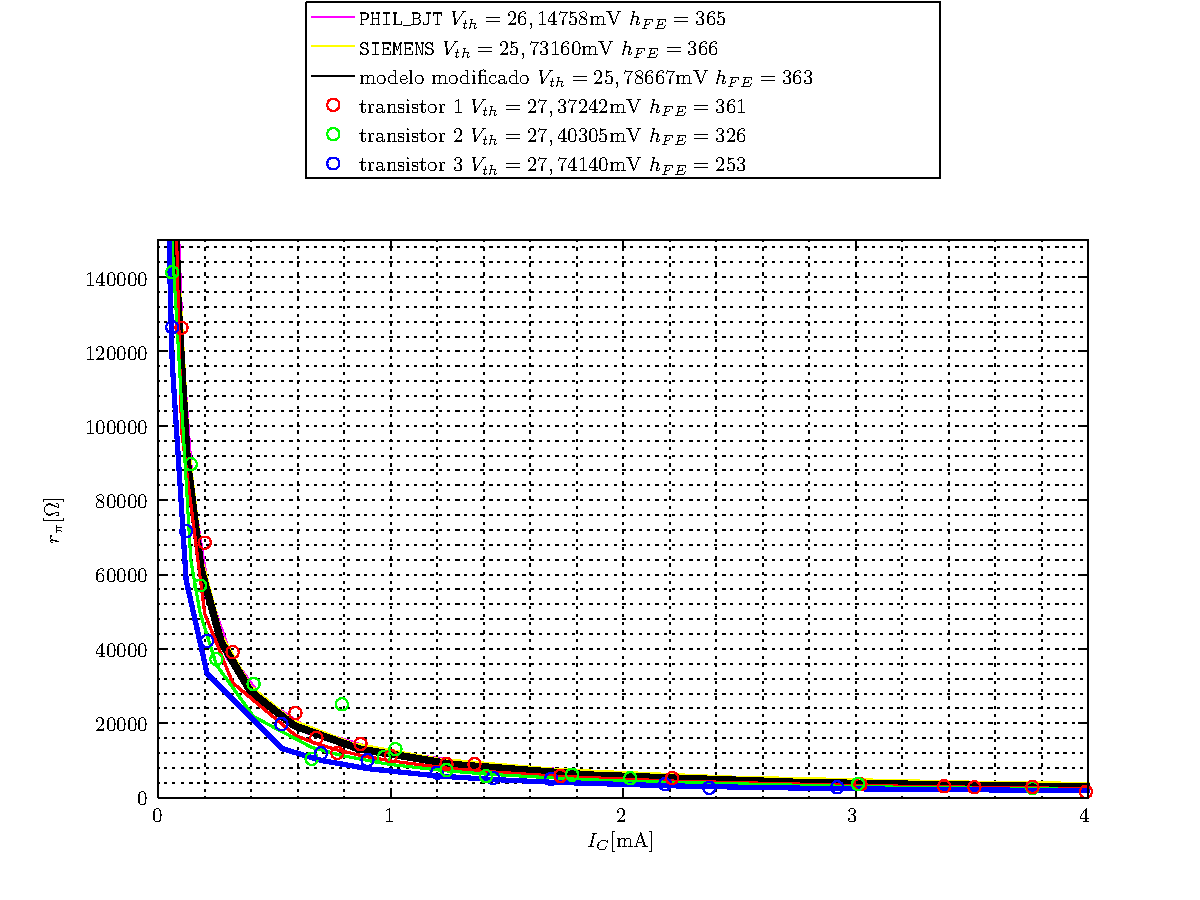
\includegraphics[scale=0.7]{./Octave/rpi.pdf}
\caption{Curva de resistencia de entrada}
 \label{fig:rpi}
\end{center}
\end{figure}

\subsection{Comparación de los resultados}

Se partió comparando los parámetros obtenidos mediante los distintos métodos
de ajuste.

De las figuras \ref{fig:transferencia_exp} y \ref{fig:transferencia_lineal}
a simple vista no se encuentra una diferencia importante entre los ajustes,
sin embargo en la tabla \ref{table:comparacion_ajuste} podemos encontrar
diferencias importantes entre los valores de $I_S$ de cada transistor para
distintos ajustes y poca diferencia entre los valores de $V_{th}$ de cada
transistor para distintos distintos ajustes.

\begin{table}[H]
\centering
\begin{tabular}{|c|c|c|c|c|c|c|}
\hline
& \texttt{PHIL\_BJT} & \texttt{SIEMENS} & modelo modificado & Transistor 1 & Transistor 2 & Transistor 3 \\
\hline
$\abs{\frac{I_{S_{exp}} - I_{S_{lineal}}}{I_{S_{exp}}}}\ 100 \%$ & $ 16,4\%$ & $ 33,3\%$ & $3,7 \%$ & $40,7 \%$ & $68,7 \%$ & $28,4 \%$\\
\hline
$\abs{\frac{V_{th_{exp}} - V_{th_{lineal}}}{V_{th_{exp}}}}\ 100 \%$ & $0,8 \%$ & $1,8 \%$ & $0,3 \%$ & $1,6 \%$ & $5,1 \%$ & $1,2 \%$\\
\hline
\end{tabular}
\caption{Comparación entre los dos métodos de ajuste}
\label{table:comparacion_ajuste}
\end{table}

Se puede apreciar que la corriente de saturación para cada transistor 
son muy similares. Esto habla de la construcción de los dispositivos, 
los parámetros constructivos deben ser similares para que esto ocurra.

Finalmente comparamos los parámetros principales de los transistores
simulados con el transistor 1.
En la tabla \ref{table:comparacion_simulaciones}
se eligió el transistor 1 como referencia ya que el modelo modificado
fue diseñado con sus parámetros principales.

\begin{table}[H]
\centering
\begin{tabular}{c|c|c|c|c|l}
\cline{2-5}
& $X$ & \texttt{PHIL\_BJT} & \texttt{SIEMENS} & modelo modificado \\ 
\cline{1-5}
\multicolumn{1}{ |c|  }{\multirow{2}{*}{Ajuste exponencial} } & $\abs{\frac{I_{S_{X}} - I_{S_{transistor\ 1}}}{I_{S_{transistor\ 1}}}} \ 100 \%$  & $23,7\%$ & $60,4\%$ & $43,4\%$ &\\ 
\cline{2-5}
\multicolumn{1}{ |c|  }{} & $\abs{\frac{V_{th_{X}} - V_{th_{transistor\ 1}}}{V_{th_{transistor\ 1}}}} \ 100 \%$  & $2,2\%$ & $2,8\%$ & $4,0\%$ &\\ 
\cline{1-5}
\multicolumn{1}{ |c|  }{\multirow{2}{*}{Ajuste lineal} } & $\abs{\frac{I_{S_{X}} - I_{S_{transistor\ 1}}}{I_{S_{transistor\ 1}}}} \ 100 \%$  & $54,7\%$ & $81,2\%$ & $2,5\%$ &\\ 
\cline{2-5}
\multicolumn{1}{ |c|  }{} & $\abs{\frac{V_{th_{X}} - V_{th_{transistor\ 1}}}{V_{th_{transistor\ 1}}}} \ 100 \%$  & $4,5\%$ & $6,0\%$ & $5,8\%$ &\\ 
\cline{1-5}
\multicolumn{1}{ |c|  }{\multirow{2}{*}{$I_C \approx 5\unit{mA}$ }} & $  \abs{\frac{r_{o_{X}} - r_{o_{transistor\ 1}}}{r_{o_{transistor\ 1}}}} \ 100 \%$  & $45,3\%$ & $8,5\%$ & $13,2\%$ &\\ 
\cline{2-5}
\multicolumn{1}{ |c|  }{} & $  \abs{\frac{V_{A_{X}} - V_{A_{transistor\ 1}}}{V_{A_{transistor\ 1}}}} \ 100 \%$  & $40,2\%$ & $2,2\%$ & $4,6\%$ &\\ 
\cline{1-5}
\multicolumn{1}{ |c|  }{\multirow{2}{*}{$I_C \approx 25\unit{mA}$ }} & $  \abs{\frac{r_{o_{X}} - r_{o_{transistor\ 1}}}{r_{o_{transistor\ 1}}}} \ 100 \%$  & $52,2\%$ & $146,0\%$ & $115,0\%$ &\\ 
\cline{2-5}
\multicolumn{1}{ |c|  }{} & $  \abs{\frac{V_{A_{X}} - V_{A_{transistor\ 1}}}{V_{A_{transistor\ 1}}}} \ 100 \%$  & $43,8\%$ & $145,2\%$ & $172,5\%$ &\\ 
\cline{1-5}
\end{tabular}
\caption{Comparación de los parámetros principales de los modelos simulados respecto al transistor 1}
\label{table:comparacion_simulaciones}
\end{table}

En las curvas de salida se encontró que para los transistores utilizados
en las mediciones experimentales el parámetro $V_A$ varía respecto a la
corriente a la que satura el colector $I_{C_{MAD}}$. Esto no ocurre en
los transistores simulados en \emph{Spice}.\\
También como se puede observar en la figura \ref{fig:salida_5ma} en todos
los transistores la corriente $I_C$ satura aproximadamente a la misma tensión $V_{CE} \approx 300\unit{mV}$
como fué indicado en las hojas de datos.
Esto no ocurre para $I_{C_{MAD}} \approx 25 \unit{mA}$, como se puede observar
en la figura \ref{fig:salida_25ma}, en donde la corriente de los transistores
simulados satura a $V_{CE} \approx 300\unit{mV}$ y la corriente de los transistores
medidos satura a $V_{CE} \approx 1400\unit{mV}$.

\section{Conclusión}

Entre los distintos métodos de ajuste, para las curvas de transferencia,
podemos concluir que el parámetro $I_S$ no tiene mucha influencia en la curva.
Ya que a pesar de tener diferencias importantes entre distintos métodos
de ajustes las curvas son muy similares.
No hubo diferencias importantes entre los valores de $V_{th}$ tanto 
para los transistores usados en las mediciones experimentales como en los 
simulados. Esto corroboró que $V_{th}$ depende de la temperatura ya que
$V_{th} = \frac{K\ T}{q}$ y al estar los transistores aproximadamente
a la misma temperatura los valores obtenidos fueron similares.

Se encontraron más diferencias entre las curvas simuladas con las
obtenidas experimentalmente para $I_{C_{MAD}} \approx 25 \unit{mA}$ que para
$I_{C_{MAD}} \approx 5 \unit{mA}$. Con lo que se puede concluir que
a mayores valores de $I_{C}$ los datos experimentales varían respecto
a los valores obtenidos mediante las simulaciones en \emph{Spice} y los
datos obtenidos de las hojas de datos.

Respecto a la transconductancia $g_m$ se pudo observar en los gráficos
que a medida que $I_C$ auenta el valor teórico difiere del experimental.


Finalmente destacamos que a partir de lo observado no es posible diseñar 
precisamente un circuito a partir de la información proveniente de las hojas de datos
dado que el parámetro $h_{FE}$ en los transistores
TBJ tiene valores muy diversos para transistores del mismo modelo.
Esto se debe a que es difícil de controlar en el proceso de fabricación.
Es importante considerarlo ya que para  conseguir los mismos resultados con 
distintos transistores se debe modificar el circuito al que se encuentra conectado. 
Por esta misma razón para distintos transistores se debió utilizar distintas resistencias para 
obtener la misma corriente de saturación durante las mediciones experimentales.

\end{document}
